%%%%%%%%%%%%%%%%%%%%%%%%%%%%%%%%%%%%%%%%%%%%%%%%%%%%%%%%%%%%%%%%%%%%%%%%%%%%%%%%%%%%
%% Para começar a usar este template, na plataforma ShareLatex,                   %%
%% vá nas opções no canto esquerdo superior da tela e clique em "Copiar Projeto"  %%
%% e dê um novo nome para o projeto.                                              %%
%%                                                                                %%
%% Customizações do abnTeX2 (http://abnTeX2.googlecode.com)                       %%
%% para a Universidade Federal do Ceara - UFC                                     %%
%%                                                                                %%
%% This work may be distributed and/or modified under the                         %% 
%% conditions of the LaTeX Project Public License, either version 1.3             %%
%% of this license or (at your option) any later version.                         %%
%% The latest version of this license is in                                       %%
%%   http://www.latex-project.org/lppl.txt                                        %%
%% and version 1.3 or later is part of all distributions of LaTeX                 %%
%% version 2005/12/01 or later.                                                   %%
%%                                                                                %%
%% This work has the LPPL maintenance status `maintained'.                        %%
%%                                                                                %%
%% The Currentt Maintainer of this work are Ednardo Moreira Rodrigues (UFC/DEE)   %%
%% and Alan Batista de Oliveira (UFC/DEE)                                         %%
%%                                                                                %%
%% Review:                                                                        %%
%%                                                                                %%
%% - Eliene Maria Vieira de Moura;                                                %%
%% - Francisco Edvander Pires Santos;                                             %%
%% - Izabel Lima dos Santos;                                                      %%
%% - Juliana Soares Lima;                                                         %%
%% - Kalline Yasmin Soares Feitosa.                                               %%
%%                                                                                %%
%% The First Maintainer of this work was Thiago Nascimento  (UECE)                %%
%% Project available on: https://github.com/thiagodnf/uecetex2                    %%
%%                                                                                %%
%% Further information about abnTeX2                                              %%
%% are available on http://abntex2.googlecode.com/                                %%
%%                                                                                %%
%%%%%%%%%%%%%%%%%%%%%%%%%%%%%%%%%%%%%%%%%%%%%%%%%%%%%%%%%%%%%%%%%%%%%%%%%%%%%%%%%%%%

\documentclass[        
    a4paper,          % Tamanho da folha A4
    12pt,             % Tamanho da fonte 12pt
    chapter=TITLE,    % Todos os capitulos devem ter caixa alta
    section=Title,    % Todas as secoes devem ter caixa alta somente na primeira letra
    subsection=Title, % Todas as subsecoes devem ter caixa alta somente na primeira letra
    oneside,          % Usada para impressao em apenas uma face do papel
    english,          % Hifenizacoes em ingles
    spanish,          % Hifenizacoes em espanhol
    brazil,           % Ultimo idioma eh o idioma padrao do documento
    fleqn             % Coloca as equações alinhadas a esquerda
]{abntex2}

%%%%%%%%%%%%%%%%%%%%%%%%%%%%%%%%%%%%%%%%%%%%%%%%%%%%%%%%%%%%%%%%%%%%%%%%%%
%% Customizações do abnTeX2 (http://abnTeX2.googlecode.com)             %%
%% para a Universidade Federal do Ceara - UFC                           %%
%%                                                                      %%
%% This work may be distributed and/or modified under the               %% 
%% conditions of the LaTeX Project Public License, either version 1.3   %%
%% of this license or (at your option) any later version.               %%
%% The latest version of this license is in                             %%
%%   http://www.latex-project.org/lppl.txt                              %%
%% and version 1.3 or later is part of all distributions of LaTeX       %%
%% version 2005/12/01 or later.                                         %%
%%                                                                      %%
%% This work has the LPPL maintenance status `maintained'.              %%
%%                                                                      %%
%% The Currentt Maintainer of this work are Ednardo Rodrigues (UFC/DEE) %%
%% and Alan Batista (UFC/DEE)                                           %%
%%                                                                      %%
%% Review:                                                              %%
%%                                                                      %%
%% - Eliene Maria Vieira de Moura;                                      %%
%% - Francisco Edvander Pires Santos;                                   %%
%% - Izabel Lima dos Santos;                                            %%
%% - Juliana Soares Lima;                                               %%
%% - Kalline Yasmin Soares Feitosa.                                     %%
%%                                                                      %%
%% The First Maintainer of this work was Thiago Nascimento  (UECE)      %%
%% Project available on: https://github.com/thiagodnf/uecetex2          %%
%%                                                                      %%
%% Further information about abnTeX2                                    %%
%% are available on http://abntex2.googlecode.com/                      %%
%%                                                                      %%
%%%%%%%%%%%%%%%%%%%%%%%%%%%%%%%%%%%%%%%%%%%%%%%%%%%%%%%%%%%%%%%%%%%%%%%%%%

% \documentclass[        
%     a4paper,          % Tamanho da folha A4
%     12pt,             % Tamanho da fonte 12pt
%     chapter=TITLE,    % Todos os capitulos devem ter caixa alta
%     section=TITLE,    % Todas as secoes devem ter caixa alta
%     oneside,          % Usada para impressao em apenas uma face do papel
%     english,          % Hifenizacoes em ingles
%     spanish,          % Hifenizacoes em espanhol
%     brazil            % Ultimo idioma eh o idioma padrao do documento
% ]{abntex2}

% Importações de pacotes
\usepackage[utf8]{inputenc}                         % Acentuação direta
\usepackage[T1]{fontenc}                            % Codificação da fonte em 8 bits
\usepackage{graphicx}                               % Inserir figuras
\usepackage{amsfonts, amssymb, amsmath}             % Fonte e símbolos matemáticos
\usepackage{booktabs}                               % Comandos para tabelas
\usepackage{verbatim}                               % Texto é interpretado como escrito no documento
\usepackage{multirow, array}                        % Múltiplas linhas e colunas em tabelas
\usepackage{indentfirst}                            % Endenta o primeiro parágrafo de cada seção.
\usepackage{listings}                               % Utilizar codigo fonte no documento
\usepackage{xcolor}
\usepackage{microtype}                              % Para melhorias de justificação?
\usepackage[portuguese,ruled,lined]{algorithm2e}    % Escrever algoritmos
\usepackage{algorithmic}                            % Criar Algoritmos  
%\usepackage{float}                                  % Utilizado para criação de floats
\usepackage{amsgen}
\usepackage{lipsum}                                 % Usar a simulação de texto Lorem Ipsum
%\usepackage{titlesec}                               % Permite alterar os títulos do documento
\usepackage{tocloft}                                % Permite alterar a formatação do Sumário
\usepackage{etoolbox}                               % Usado para alterar a fonte da Section no Sumário
\usepackage[nogroupskip,nonumberlist]{glossaries}                % Permite fazer o glossario
\usepackage[font=singlespacing]{caption}                                % Altera o comportamento da tag caption
\usepackage[alf, abnt-emphasize=bf, recuo=0cm, abnt-etal-cite=2, abnt-etal-list=0, abnt-etal-text=it]{abntex2cite}  % Citações padrão ABNT
%\usepackage[bottom]{footmisc}                      % Mantém as notas de rodapé sempre na mesma posição
%\usepackage{times}                                 % Usa a fonte Times
\usepackage{mathptmx}                               % Usa a fonte Times New Roman										
%\usepackage{lmodern}                               % Usa a fonte Latin Modern
%\usepackage{subfig}                                % Posicionamento de figuras
%\usepackage{scalefnt}                              % Permite redimensionar tamanho da fonte
%\usepackage{color, colortbl}                       % Comandos de cores
%\usepackage{lscape}                                % Permite páginas em modo "paisagem"
%\usepackage{ae, aecompl}                           % Fontes de alta qualidade
%\usepackage{picinpar}                              % Dispor imagens em parágrafos
%\usepackage{latexsym}                              % Símbolos matemáticos
%\usepackage{upgreek}                               % Fonte letras gregas
\usepackage{appendix}                               % Gerar o apendice no final do documento
\usepackage{paracol}                                % Criar paragrafos sem identacao
\usepackage{lib/ufctex}		                        % Biblioteca com as normas da UFC para trabalhos academicos
\usepackage{pdfpages}                               % Incluir pdf no documento
\usepackage{amsmath}                                % Usar equacoes matematicas

% Organiza e gera a lista de abreviaturas, simbolos e glossario
\makeglossaries

% Gera o Indice do documento
\makeindex


%%%%%%%%%%%%%%%%%%%%%%%%%%%%%%%%%%%%%%%%%%%%%%%%%%%%%
%%          Configuracoes do ufctex                %%
%%%%%%%%%%%%%%%%%%%%%%%%%%%%%%%%%%%%%%%%%%%%%%%%%%%%%

% Opcoes disponiveis

\trabalhoacademico{tccgraduacao}
%\trabalhoacademico{tccespecializacao}
%\trabalhoacademico{dissertacao}
%\trabalhoacademico{tese}

% Define se o trabalho eh uma qualificacao
% Coloque 'nao' para versao final do trabalho

\ehqualificacao{nao}

% Remove as bordas vermelhas e verdes do PDF gerado
% Coloque 'sim' pare remover

\removerbordasdohyperlink{sim} 

% Adiciona a cor Azul a todos os hyperlinks

\cordohyperlink{nao}

%%%%%%%%%%%%%%%%%%%%%%%%%%%%%%%%%%%%%%%%%%%%%%%%%%%%%
%%          Informação sobre a IES                 %%
%%%%%%%%%%%%%%%%%%%%%%%%%%%%%%%%%%%%%%%%%%%%%%%%%%%%%

\ies{Universidade Federal do Ceará}
\iessigla{UFC}
\centro{SEMINÁRIO DE MONOGRAFIA}

%%%%%%%%%%%%%%%%%%%%%%%%%%%%%%%%%%%%%%%%%%%%%%%%%%%%%
%%        Informação para TCC de Graduacao %%
%%%%%%%%%%%%%%%%%%%%%%%%%%%%%%%%%%%%%%%%%%%%%%%%%%%%%

\graduacaoem{Engenharia da computação}
\habilitacao{bacharel} % Pode colocar tambem 'licenciada'

\autor{GABRIEL DE SOUZA NOGUEIRA DA SILVA}
\titulo{Sistema de autoavaliação - PPGEEC/UFC}
\data{2021}
\local{Sobral}

% Exemplo: \dataaprovacao{01 de Janeiro de 2012}
\dataaprovacao{}

%%%%%%%%%%%%%%%%%%%%%%%%%%%%%%%%%%%%%%%%%%%%%
%%     Informação sobre o Orientador       %%
%%%%%%%%%%%%%%%%%%%%%%%%%%%%%%%%%%%%%%%%%%%%%

\orientador{Prof. Dr. Iális Cavalcante de Paula Júnior}
\orientadories{Universidade Federal do Ceará (UFC)}
\orientadorcentro{Centro de Ciências e Tecnologia (CCT)}
\orientadorfeminino{nao} % Coloque 'sim' se for do sexo feminino

%%%%%%%%%%%%%%%%%%%%%%%%%%%%%%%%%%%%%%%%%%%%%
%%      Informação sobre o Co-orientador   %%
%%%%%%%%%%%%%%%%%%%%%%%%%%%%%%%%%%%%%%%%%%%%%

% Deixe o nome do coorientador em branco para remover do documento

\coorientador{}
\coorientadories{Universidade Co-orientador (SIGLA)}
\coorientadorcentro{Centro do Co-orientador (SIGLA)}
\coorientadorfeminino{nao} % Coloque 'sim' se for do sexo feminino

%%%%%%%%%%%%%%%%%%%%%%%%%%%%%%%%%%%%%%%%%%%%%
%%      Informação sobre a banca           %%
%%%%%%%%%%%%%%%%%%%%%%%%%%%%%%%%%%%%%%%%%%%%%

% Atenção! Deixe o nome do membro da banca para remover da folha de aprovacao

% Exemplo de uso:
% \membrodabancadois{Prof. Dr. Fulano de Tal}
% \membrodabancadoisies{Universidade Federal do Ceará - UFC}

\begin{document}	

	% Elementos pré-textuais
	\imprimircapa
	\imprimirfolhaderosto{}
	
% 	\imprimirlistadeilustracoes
	\imprimirlistadetabelas
	%\imprimirlistadequadros
	%\imprimirlistadealgoritmos
	%\imprimirlistadecodigosfonte
	\imprimirlistadeabreviaturasesiglas
% 	\imprimirlistadesimbolos{elementos-pre-textuais/lista-de-simbolos}   
	\imprimirsumario
	
	%Elementos textuais
	\textual
	\chapter{Introdução}
\label{cap:introducao}

%Para começar a usar este \textit{template}, na plataforma \textit{ShareLatex}, vá nas opções (três barras vermelhas horizontais) no canto esquerdo superior da tela e clique em "Copiar Projeto" e dê um novo nome para o projeto. 
    
    Desde a implantação da pós-graduação no Brasil nos moldes definidos pelo
Parecer CFE 977/1965, a pós-graduação stricto sensu avançou no sentido do seu
crescimento numérico e no desenvolvimento de um sistema de avaliação que recebeu
aprovação da comunidade acadêmica nacional e internacional \cite{capes2019}.

    A avaliação externa assegura padrões básicos, o que é importante
em um país continental, mas tem limitações. Uma delas é o fato de não ser formativa,
em que os que estão no processo se envolvam também na solução dos problemas
identificados. Neste sentido, a autoavaliação favorece a construção da identidade,
heterogeneidade e envolvimento dos programas avaliados, para além dos padrões
mínimos garantidos pela avaliação externa.
 \cite{capes2019}.
    
    Dito isto, é de suma importância para a evolução de um programa como o \gls{PPGEEC}, que exista um sistema que tenha a possibilidade de se autoavaliar, tanto para os docentes que transmitem o conhecimento, quanto para os discentes que o recebem. Com isso, aumentando a qualidade com que o ensino é passado/recebido pelos participantes.

% Neste \textit{template}, o autor irá encontrar diversas instruções e exemplos dos recursos do uso do \textit{Latex} na plataforma \textit{ShareLatex}. O LaTeX foi desenvolvido, inicialmente, na década de 80, por Leslie Lamport e é utilizado amplamente na produção de textos matemáticos e científicos, devido a sua alta qualidade tipográfica \cite{goossens1994latex}. 

%Testando o símbolo $\symE$

%\lipsum[5]  % Simulador de texto, ou seja, é um gerador de lero-lero.

%	\begin{alineas}
%		\item Lorem ipsum dolor sit amet, consectetur adipiscing elit. Nunc dictum sed tortor nec viverra.
%		\item Praesent vitae nulla varius, pulvinar quam at, dapibus nisi. Aenean in commodo tellus. Mauris molestie est sed justo malesuada, quis feugiat tellus venenatis.
%		\item Praesent quis erat eleifend, lacinia turpis in, tristique tellus. Nunc dictum sed tortor nec viverra.
%		\item Mauris facilisis odio eu ornare tempor. Nunc dictum sed tortor nec viverra.
%		\item Curabitur convallis odio at eros consequat pretium.
%	\end{alineas}
	

	

	\chapter{OBJETIVOS}
\label{cap:objetivos}

    \section{Objetivos Gerais}
    \label{sec:objetivos-gerais}

       Desenvolver aplicativo funcional que permita a implementação do sistema de autoavaliação do \gls{PPGEEC}.
    \section{Objetivos Específicos}
    \label{sec:objetivos-especificos}
       \begin{alineascomponto}
        	\item Organizar dados, fichas de avaliação e legislação do sistema de autoavaliação do \gls{PPGEEC}.
        	\item Implantar a infra-estrutura para aplicação do sistema de autoavaliação.
        	\item Validar o desenvolvimento do sistema junto aos seus potenciais usuários.
        % 	\begin{subalineascomponto}
        % 		\item Integer non lacinia magna. Aenean tempor lorem tellus, non sodales nisl commodo ut
        % 		\item Proin mattis placerat risus sit amet laoreet.
        % 	\end{subalineascomponto}
        \end{alineascomponto}
        
        %Mais exemplos e opções de citações podem ser encontradas em:
        
%        https://en.wikibooks.org/wiki/LaTeX/Bibliography_Management
%        https://github.com/cfgnunes/latex-cefetmg/blob/master/latex-cefetmg/03-elementos-pos-textuais/apendices.tex        
        
        

%     \section{Inserindo figuras}
%     \label{sec:figuras}
    
%     A Figura \ref{fig:reitoria} apresenta a fotografia da reitoria da Universidade Federal do Ceará. Observe a estrutura do código para inserir a Figura \ref{fig:reitoria}. No título, apenas a primeira letra da frase é maiúscula  exceto nomes próprios e não há ponto final. Procure ajustar o tamanho da figura para preencher a largura delimitada pelas margens esquerda e direita. Não esqueça de indicar fonte da figura. 
    
% \begin{figure}[h!]
%     \Caption{\label{fig:reitoria} Fotografia da Reitoria da Universidade Federal do Ceará}
%     %\centering
%     \UFCfig{}{
%         \fbox{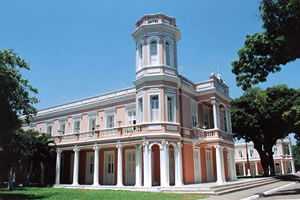
\includegraphics[width=12cm]{figuras/exemplo-1}}
%     }{
%     \Fonte{\citeonline{UFC2012}.}
%     }	
% \end{figure}

% \begin{figure}[!ht]
%     \centering
%     \caption{Fluxograma do experimento do tipo}
%     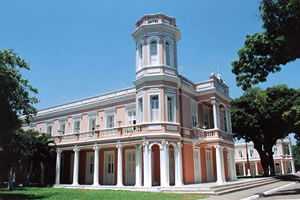
\includegraphics[width=0.9\textwidth]{figuras/exemplo-1}
%     \Fonte{Elaborado pelo autor.}
%     \label{fig:np_np}
% \end{figure}

%     Texto texto texto texto texto texto texto texto texto texto texto texto texto texto texto texto texto texto texto texto texto texto texto texto texto texto texto texto texto texto texto texto texto texto texto texto texto texto texto texto texto texto texto texto texto.

%     Texto texto texto texto texto texto texto texto texto texto texto texto texto texto texto texto texto texto texto. Texto texto texto texto texto texto texto texto texto texto texto texto texto texto texto texto texto texto texto.

%     A Figura \ref{fig:sondas} Texto texto texto texto texto texto texto texto texto texto texto texto texto texto texto texto texto texto texto. Texto texto texto texto texto texto texto texto texto texto texto texto texto texto texto texto texto texto texto.

% 	\begin{figure}[h!]
% 		\centering
% 		\Caption{\label{fig:sondas} Gráfico da Atmosfera Superior}	
% 		\UFCfig{}{
% 			\fbox{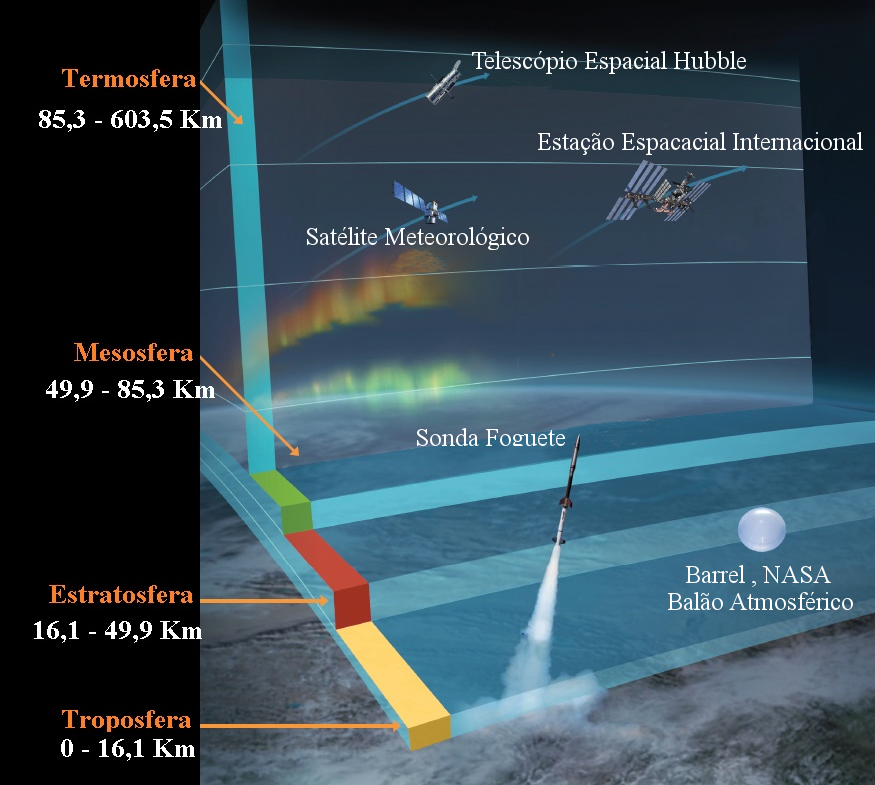
\includegraphics[width=12cm]{figuras/sondas}}
% 		}{
% 			\Fonte{adaptado de \citeonline{NASA2016}.}}	
% 	\end{figure}

%     Texto texto texto texto texto texto texto texto texto texto texto texto texto texto texto texto texto texto texto texto texto texto texto texto texto texto texto texto texto texto texto texto texto texto texto texto texto texto texto texto texto texto texto texto texto.

%     Texto texto texto texto texto texto texto texto texto texto texto texto texto texto texto texto texto texto texto texto texto texto texto texto texto texto texto texto texto texto texto texto texto texto texto texto texto texto texto texto texto texto texto texto texto.

%     Texto texto texto texto texto texto texto texto texto texto texto texto texto texto texto texto texto texto texto texto texto texto texto texto texto texto texto texto texto texto texto texto texto texto texto texto texto texto texto texto texto texto texto texto texto.

%     Texto texto texto texto texto texto texto texto texto texto texto texto texto texto texto texto texto texto texto texto texto texto texto texto texto texto texto texto texto texto texto texto texto texto texto texto texto texto texto texto texto texto texto texto texto.

%     Texto texto texto texto texto texto texto texto texto texto texto texto texto texto texto texto texto texto texto texto texto texto texto texto texto texto texto texto texto texto texto texto texto texto texto texto texto texto texto texto texto texto texto texto texto.

%     \section{Inserindo tabelas}
%     \label{sec:tabelas}

% 	A Tabela \ref{tab:exemplo-1} Texto texto texto texto texto texto texto texto texto texto texto texto texto texto texto texto texto texto texto. Texto texto texto texto texto texto texto texto texto texto texto texto texto texto texto texto texto texto texto.

% \subsection{Exemplo de subseção} \label{sec:ex_sec}
	
% Texto texto texto texto texto texto texto texto texto texto texto texto texto texto texto texto texto texto texto texto texto texto texto texto texto texto texto texto texto texto texto texto texto texto texto texto texto texto texto texto texto texto texto texto texto.

% %acrlong{DATASUS},\acrlong{DNV},\acrlong{DO},\acrlong{ESF},\acrlong{IBGE},\acrlong{MFC},\acrlong{MI},\acrlong{MS},\acrlong{NV},\acrlong{ODM},\acrlong{OI},\acrlong{OMS},\acrlong{ONU},\acrlong{PNI},\acrlong{PSF},\acrlong{RIPSA},\acrlong{RN},\acrlong{SIM},\acrlong{SINASC},\acrlong{SUS},\acrlong{TMI},\acrlong{TMMFC}


% \begin{alineascomponto}
% 	\item Integer non lacinia magna. Aenean tempor lorem tellus, non sodales nisl commodo ut
% 	\item Proin mattis placerat risus sit amet laoreet. Praesent sapien arcu, maximus ac fringilla efficitur, vulputate faucibus sem. Donec aliquet velit eros, sit amet elementum dolor pharetra eget
% 	\item Integer eget mattis libero. Praesent ex velit, pulvinar at massa vel, fermentum dictum mauris. Ut feugiat accumsan augue, et ultrices ipsum euismod vitae
% 	\begin{subalineascomponto}
% 		\item Integer non lacinia magna. Aenean tempor lorem tellus, non sodales nisl commodo ut
% 		\item Proin mattis placerat risus sit amet laoreet.
% 	\end{subalineascomponto}
% \end{alineascomponto}

% Teste de siglas \gls{TMMFC}
	\chapter{JUSTIFICATIVA}
\label{cap:justificativa}
   Diante de toda informação apresentada, pode-se perceber que a tecnologia proposta traz benefícios tanto para o programa que o adota, quanto para os docentes e discente que o utilizam, podendo usufruir de \textit{feedbacks} para o melhor funcionamento. Sendo assim, o desenvolvimento de uma aplicação capaz de fazer com que os docente, discentes e técnicos administrativos possam tanto avaliar o programa como um todo, quanto disciplinas e o desempenho dos docentes e se autoavaliar, se torna de suma importância para e evolução e criação de um programa melhor para todos os envolvidos.

    
        


	\chapter{MATERIAIS E MÉTODOS}
\label{cap:materiais-e-metodos}
   Para o desenvolvimento do projeto apresentado, será necessário o conhecimento da linguagem de programação javascript, linguagem SQL. Além disso, será utilizado a biblioteca Node.js para o desenvolvimento do \textit{Backend} da aplicação, bem como a biblioteca ReactJs e do framework React-Admin para a construção de um painel administrativo (\textit{Frontend}). Além disso, para solucionar de forma eficiente o problema atual será utilizado as orientações presentes na RESOLUÇÃO Nº 1/2021/CMEEC/CUFCSOBRAL/REITORIA \cite{resolucao2021}.
    
    \section{Linguagem SQL}
    \label{sec:sql}

        Será utilizada para criação do banco de dados PostgreSQL, onde será armazenado todos os dados de usuários, bem como suas respostas das autoavaliações realizadas. Nesse caso de uso, a sua principal vantagem, é a capacidade de relacionar os usuários a suas funções especificas (docentes, discentes e técnicos administrativos) e suas devidas propriedades. 
    
    \section{Node.js}
    \label{sec:node.js}
        Será utilizado para criação do \textit{Backend} da aplicação. Nesse caso, estarei desenvolvendo uma \gls{API} onde será disponibilizado rotas no formato \gls{HTTP} (\textit{GET}, \textit{POST}, \textit{UPDATE} e \textit{DELETE}), onde as informações trafegam pela rede no formato de \gls{JSON}, para ser consumido pelos \textit{Frontends}.\nocite{docnode2021}
        
    \section{ReactJs e React-Admin}
    \label{sec:reactjs}
        Será utilizado para criação do \textit{Frontend} da aplicação. Nesse caso, será desenvolvido o painel administrativo da aplicação, onde será possível manipular dados de usuários, fichas e disciplinas.\nocite{docreact2021}\nocite{docreactadmin2021}

    \section{Resolução do PPGEEC}
    \label{sec:reactjs}
        Será utilizado para orientar o processo de desenvolvimento do software, pois as fichas de autoavaliação devem seguir as normas indicadas nessa resolução. Dito isto, as fichas serão o instrumento para a autoavaliação do programa, sendo elas compostas por perguntas que terão as seguintes opções: Ótimo, Bom, Regular, Ruim, Péssimo, Não conheço e Não se aplica. Dessa forma, somente uma opção é permitida como resposta. Com isso, o tema de cada ficha será um dos seguintes: Ficha de avaliação da secretaria, Ficha de avaliação da coordenação, Ficha de avaliação dos discentes em relação aos docentes (disciplinas), Ficha de avaliação dos discentes em relação aos docentes (orientações), Ficha de avaliação dos docentes em relação ao desempenho dos discentes das disciplinas ministradas,
        Ficha de avaliação dos docentes em relação ao desempenho dos discentes nas orientações, Ficha de avaliação das disciplinas,
        Ficha de avaliação da banca de dissertação, Ficha de avaliação de eventos (quando ocorrerem),
        Ficha de avaliação do egresso sobre o desempenho do PPGEEC e Ficha de avaliação da infraestrutura.
	\chapter{Metodologia}
\label{chap:metodologia}

Ao longo desta seção serão descritos e detalhados as etapas para a metodologia proposta para o desenvolvimento da aplicação proposta.

\section{Levantamento de requisitos com a coordenação do programa}
\label{sec:requisitos}
Inicialmente, foi realizado um levantamento de quais seriam os pontos relevantes para que o programa tivesse um impacto positivo e cumprisse seu papel. Dito isso, ocorrerá uma sequencia de reuniões com a coordenação e responsáveis, para melhor atender a demanda e levantamento de requisitos obrigatórios e opcionais na primeira versão da aplicação.
\section{Desenvolvimento do \textit{Backend}}
\label{sec:backend}
Após os requisitos estarem claros darei inicio, a modelagem do banco de dados que irá armazenar todas as respostas dos usuários, bem como suas informações. Por conseguinte, seguirei com o desenvolvimento de uma \gls{API}, onde teremos rotas especificas para cada cada funcionalidade, fazendo com que possa ser consumida por uma interface web ou mobile com facilidade.
\section{Desenvolvimento do \textit{Frontend} de administração}
\label{sec:frontend}
Em paralelo com a construção do \textit{Backend}, estarei desenvolvendo o painel administrativo, onde será possível a criar, listar, atualizar e deletar, as entidades acordadas no inicio do projeto.

\section{Cronograma}
\label{sec:cronograma}
 
\begin{table}[h!]
	\Caption{\label{tabela-desenvolvimento} Cronograma de previsão de desenvolvimento do projeto (2021)}%
	\IBGEtab{}{%
		\begin{tabular}{cccccc}
			\toprule
			Etapa & Setembro & Outubro & Novembro & Dezembro & Janeiro \\
			\midrule \midrule
			1 & x &  & & &  \\
			2 &  & x & & & \\
			3 & & & x & &\\
			4 & & & & x &\\
			5 & & & & & x\\
			\bottomrule
		\end{tabular}%
	}{%
	\Fonte{Elaborado pelo autor.}%
% 	\Nota{esta é uma nota, que diz que os dados são baseados na
% 		regressão linear.}%
% 	\Nota[Anotações]{uma anotação adicional, seguida de várias outras.}%
}
\end{table}

\begin{alineascomnumero}
    \item Colher \textit{feedbacks} do mvp rodado semestre passado e alterar onde seria necessário.
	\item Construção de novas rotas para atender as necessidades do \textit{frontend}.
	\item Refatoração do projeto.
	\item Construir testes unitários.
	\item Finalização e colocar a aplicação em produção.
\end{alineascomnumero}

% Texto texto texto texto texto texto texto texto texto texto texto.

% %\begin{algorithm}[H]
% %	\Entrada{o proprio texto}
% %	\Saida{como escrever algoritmos com \LaTeX2e }
% %	\Inicio{
% %		inicialização\;
% %		\Repita{fim do texto}{
% %			leia o atual\;
% %			\Se{entendeu}{
% %				vá para o próximo\;
% %				próximo se torna o atual\;}
% %			\Senao{volte ao início da seção\;}
% %		}
% %	}
% %	\caption{Exemplo de Algoritmo Versao 02}
% %\end{algorithm}

% %\begin{algorithm}
% %	\begin{algorithmic}
% %	\Entrada{o proprio texto}
% %	\Saida{como escrever algoritmos com \LaTeX2e }	
% %	\end{algorithmic}
% %\end{algorithm}

% Exemplo de alíneas com números:

% \begin{alineascomnumero}
% 	\item Texto texto texto texto texto texto texto texto texto texto texto texto .
% 	\item Texto texto texto texto texto texto texto texto texto texto texto texto .
% 	\item Texto texto texto texto texto texto texto texto texto texto texto texto .
% 	\item Texto texto texto texto texto texto texto texto texto texto texto texto .
% 	\item Texto texto texto texto texto texto texto texto texto texto texto texto .
% 	\item Texto texto texto texto texto texto texto texto texto texto texto texto .
% \end{alineascomnumero}

% Texto texto texto texto texto texto texto texto texto texto texto texto texto texto texto texto texto texto texto texto texto texto texto texto texto texto texto texto texto texto texto texto texto texto texto texto texto texto texto texto texto texto texto texto texto texto texto texto texto texto texto texto texto texto texto texto texto texto texto texto texto texto texto texto texto texto texto texto texto.

 


% Ou então figuras podem ser incorporadas de arquivos externos, como é o caso da \autoref{fig-grafico-1}. Se a figura que ser incluída se tratar de um diagrama, um gráfico ou uma ilustração que você mesmo produza, priorize o uso de imagens vetoriais no formato PDF. Com isso, o tamanho do arquivo final do trabalho será menor, e as imagens terão uma apresentação melhor, principalmente quando impressas, uma vez que imagens vetorias são perfeitamente escaláveis para qualquer dimensão. Nesse caso, se for utilizar o Microsoft Excel para produzir gráficos, ou o Microsoft Word para produzir ilustrações, exporte-os como PDF e os incorpore ao documento conforme o exemplo abaixo. No entanto, para manter a coerência no uso de software livre (já que você está usando LaTeX e abnTeX),  teste a ferramenta InkScape\index{InkScape}. ao CorelDraw\index{CorelDraw} ou ao Adobe Illustrator\index{Adobe! Illustrator}.  De todo modo, caso não seja possível  utilizar arquivos de imagens como PDF, utilize qualquer outro formato, como JPEG, GIF, BMP, etc.  Nesse caso, você pode tentar aprimorar as imagens incorporadas com o software livre \index{Gimp}Gimp. Ele é uma alternativa livre ao Adobe Photoshop\index{Adobe! Photoshop}.

% \section{Usando Fórmulas Matemáticas}

% A seguir, exemplos de inserção de fórmulas:
% Texto texto texto texto texto texto texto texto texto texto texto texto texto texto texto texto texto texto texto texto texto texto texto texto texto texto texto texto texto texto texto texto texto texto texto texto texto texto texto texto texto texto texto texto texto texto texto texto texto texto texto texto texto texto texto texto texto texto texto texto texto texto texto texto texto texto texto texto texto.

% 	\begin{equation}
% 		\begin{aligned}
% 			x = a_0 + \cfrac{1}{a_1
% 				+ \cfrac{1}{a_2
% 					+ \cfrac{1}{a_3 + \cfrac{1}{a_4} } } }
% 		\end{aligned}
% 	\end{equation}
	
% Texto texto texto texto texto texto texto texto texto texto texto texto texto texto texto texto texto texto texto texto texto texto texto texto texto texto texto texto texto texto texto texto texto texto texto texto texto texto texto texto texto texto texto texto texto texto texto texto texto texto texto texto texto texto texto texto texto texto texto texto texto texto texto texto texto texto texto texto texto.

% 	\begin{equation}
% 		\begin{aligned}
% 			k_{n+1} = n^2 + k_n^2 - k_{n-1}
% 		\end{aligned}
% 	\end{equation}
% Texto texto texto texto texto texto texto texto texto texto texto texto texto texto texto texto texto texto texto texto texto texto texto texto texto texto texto texto texto texto texto texto texto texto texto texto texto texto texto texto texto texto texto texto texto texto texto texto texto texto texto texto texto texto texto texto texto texto texto texto texto texto texto texto texto texto texto texto texto.

% 	\begin{equation}
% 		\begin{aligned}
% 			\cos (2\theta) = \cos^2 \theta - \sin^2 \theta
% 		\end{aligned}
% 	\end{equation}
	
% Texto texto texto texto texto texto texto texto texto texto texto texto texto texto texto texto texto texto texto texto texto texto texto texto texto texto texto texto texto texto texto texto texto texto texto texto texto texto texto texto texto texto texto texto texto texto texto texto texto texto texto texto texto texto texto texto texto texto texto texto texto texto texto texto texto texto texto texto texto.

% 	\begin{equation}
% 		\begin{aligned}
% 			A_{m,n} =
% 			\begin{pmatrix}
% 			a_{1,1} & a_{1,2} & \cdots & a_{1,n} \\
% 			a_{2,1} & a_{2,2} & \cdots & a_{2,n} \\
% 			\vdots  & \vdots  & \ddots & \vdots  \\
% 			a_{m,1} & a_{m,2} & \cdots & a_{m,n}
% 			\end{pmatrix}
% 		\end{aligned}
% 	\end{equation}

% Texto texto texto texto texto texto texto texto texto texto texto texto texto texto texto texto texto texto texto texto texto texto texto texto texto texto texto texto texto texto texto texto texto texto texto texto texto texto texto texto texto texto texto texto texto texto texto texto texto texto texto texto texto texto texto texto texto texto texto texto texto texto texto texto texto texto texto texto texto.
% 	\begin{equation}
% 		\begin{aligned}
% 			f(n) = \left\{ 
% 			\begin{array}{l l}
% 			n/2 & \quad \text{if $n$ is even}\\
% 			-(n+1)/2 & \quad \text{if $n$ is odd}
% 			\end{array} \right.
% 		\end{aligned}
% 	\end{equation}
% Texto texto texto texto texto texto texto texto texto texto texto texto texto texto texto texto texto texto texto texto texto texto texto texto texto texto texto texto texto texto texto texto texto texto texto texto texto texto texto texto texto texto texto texto texto texto texto texto texto texto texto texto texto texto texto texto texto texto texto texto texto texto texto texto texto texto texto texto texto.

% \section{Usando Algoritmos}

%  Texto texto texto texto texto texto texto texto texto texto texto texto texto texto texto texto texto texto texto texto texto texto texto texto texto texto texto texto texto texto texto texto texto texto texto texto texto texto texto texto texto texto texto texto texto texto texto texto texto texto texto texto texto texto texto texto texto texto texto texto texto texto texto texto texto texto texto texto texto.

% %\begin{algorithm}[h!]
% %	\SetSpacedAlgorithm
% %	\caption{\label{alg:algoritmo_de_colonica_de_formigas}Algoritmo de Otimização por Colônia de Formiga}
% %	\Entrada{Entrada do Algoritmo}
% %	\Saida{Saida do Algoritmo}
% %	\Inicio{
% %		Atribua os valores dos parâmetros\;
% %		Inicialize as trilhas de feromônios\;
% %		\Enqto{não atingir o critério de parada}{
% %			\Para{cada formiga}{
% %				Construa as Soluções\;
% %			}
% %			Aplique Busca Local (Opcional)\;
% %			Atualize o Feromônio\;
% %		}	
% %	}		
% %\end{algorithm}

 

% \section{Usando Código-fonte}

%  Texto texto texto texto texto texto texto texto texto texto texto texto texto texto texto texto texto texto texto texto texto texto texto texto texto texto texto texto texto texto texto texto texto texto texto texto texto texto texto texto.

% \lstinputlisting[language=C++,caption={Hello World em C++}]{figuras/main.cpp}

%  Texto texto texto texto texto texto texto texto texto texto texto texto texto texto texto texto texto texto texto texto texto texto texto texto texto texto texto texto texto texto.

% \begin{lstlisting}[language=Java,caption={Hello World em Java}]
% public class HelloWorld {
% 	public static void main(String[] args) {
% 		System.out.println("Hello World!");
% 	}
% }
% \end{lstlisting}

%  Texto texto texto texto texto texto texto texto texto texto texto texto texto texto texto texto texto texto.

% \section{Usando Teoremas, Proposições, etc}

%  Texto texto texto texto texto texto texto texto texto texto texto texto texto texto texto texto texto texto texto texto texto texto texto texto texto.

% \begin{teo}[Pitágoras]
% 	Em todo triângulo retângulo o quadrado do comprimento da
% 	hipotenusa é igual a soma dos quadrados dos comprimentos dos catetos.
% \end{teo}


% Texto texto texto texto texto texto texto texto texto texto texto texto texto texto texto.

% \begin{teo}[Fermat]
% 	Não existem inteiros $n > 2$, e $x, y, z$ tais que $x^n + y^n = z$
% \end{teo}

% Texto texto texto texto texto texto texto texto texto texto texto texto texto texto texto.

% \begin{prop}
% 	Para demonstrar o Teorema de Pitágoras...
% \end{prop}

% Texto texto texto texto texto texto texto texto texto texto texto texto texto texto texto.

% \begin{exem}
% 	Este é um exemplo do uso do ambiente exem definido acima.
% \end{exem}

% Texto texto texto texto texto texto texto texto texto texto texto texto texto texto texto.


% \begin{xdefinicao}
% 	Definimos o produto de ...
% \end{xdefinicao}

% Texto texto texto texto texto texto texto texto texto texto texto texto texto texto texto.

% \section{Usando Questões}


% Texto texto texto texto texto texto texto texto texto texto texto texto texto texto texto.


% Exemplo de elaboração de questões:
% \begin{questao}
% 	\item Esta é a primeira questão com alguns itens:
% 		\begin{enumerate}
% 			\item Este é o primeiro item
% 			\item Segundo item
% 		\end{enumerate}
% 	\item Esta é a segunda questão:
% 		\begin{enumerate}
% 			\item Este é o primeiro item
% 			\item Segundo item
% 		\end{enumerate}
% 	\item Lorem ipsum dolor sit amet, consectetur adipiscing elit. Nunc dictum sed tortor nec viverra. consectetur adipiscing elit. Nunc dictum sed tortor nec viverra.
% 		\begin{enumerate}
% 			\item consectetur
% 			\item adipiscing
% 			\item Nunc
% 			\item dictum
% 		\end{enumerate}
% \end{questao}

% 	\chapter{Resultados}
\label{chap:resultados}

Texto texto texto texto texto texto texto texto texto texto texto texto texto texto texto texto texto texto texto texto texto texto texto texto texto texto texto texto texto texto texto texto texto texto texto texto texto texto texto texto texto texto texto texto texto texto texto texto texto texto texto texto texto texto texto texto texto texto texto texto texto texto texto texto texto texto texto texto texto.

\section{Resultados do Experimento A}
\label{sec:resultados-do-experimento-a}


\begin{figure}[h!]
		\Caption{\label{fig:tensaoimpedanciahumana} Gráfico de tensão considerando a impedância humana}
		%\centering
		\UFCfig{}{
			\fbox{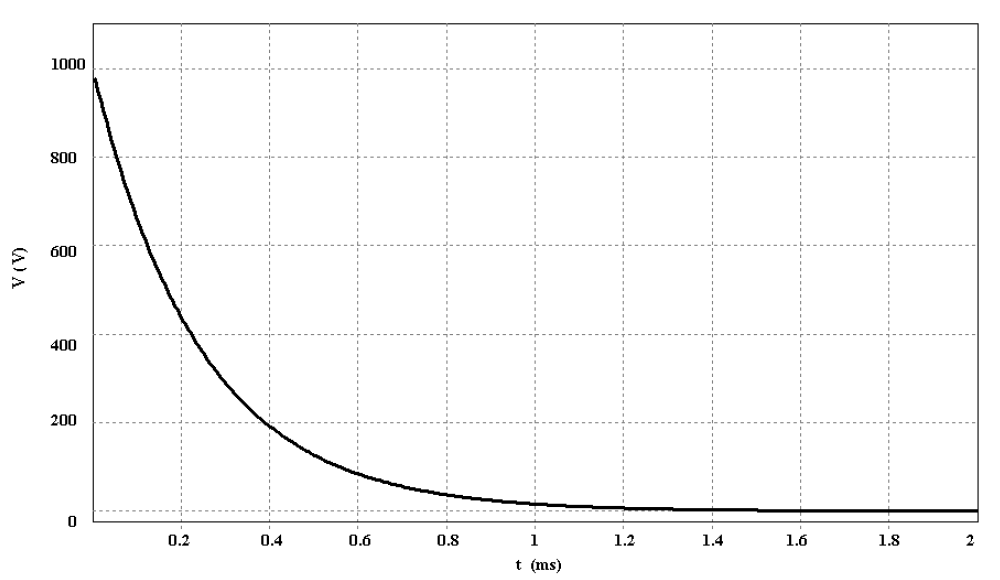
\includegraphics[width=16cm]{figuras/tensaoimpedanciahumana}}
		}{
			\Fonte{o autor.}
		}	
\end{figure}

Texto texto texto texto texto texto texto texto texto texto texto texto texto texto texto texto texto texto texto texto texto texto texto texto texto texto texto texto texto texto texto texto texto texto texto texto texto texto texto texto texto texto texto texto texto texto texto texto texto texto texto texto texto texto texto texto texto texto texto texto texto texto texto texto texto texto texto texto texto.


\begin{figure}[h!]
	\centering
	\Caption{\label{fig-grafico-1}Produção anual das dissertações de mestrado e teses de doutorado entre os anos de 1990 e 2008}		
	\IBGEtab{}{
		\fbox{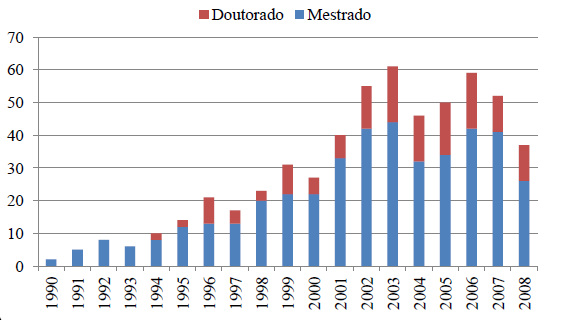
\includegraphics[width=13cm]{figuras/figura-3}}
	}{
	\Fonte{o autor}
}
\end{figure}



Texto texto texto texto texto texto texto texto texto texto texto texto texto texto texto texto texto texto texto texto texto.

Texto texto texto texto texto texto texto texto texto texto texto texto texto texto texto texto texto texto texto texto texto texto texto texto texto texto texto texto texto texto texto texto texto texto texto texto texto texto texto texto texto texto texto texto texto texto texto texto texto texto texto texto texto texto texto texto texto texto texto texto texto texto texto texto texto texto texto texto texto.

\section{Resultados do Experimento B}
\label{sec:resultados-do-experimento-b}


Texto texto texto texto texto texto texto texto texto texto texto texto texto texto texto texto texto texto texto texto texto texto texto texto texto texto texto texto texto texto texto texto ..



 Texto texto Referenciando a \autoref{tab:notas}  texto texto texto texto texto texto texto texto texto texto texto texto texto texto texto texto texto texto texto texto texto texto texto texto texto texto texto texto texto texto.Texto texto texto texto texto texto texto texto texto texto texto texto texto texto texto texto texto texto texto texto texto.

Texto texto texto texto texto texto texto texto texto texto texto texto texto texto texto texto texto texto texto texto texto texto texto texto texto texto texto texto texto texto texto texto texto texto texto texto texto texto texto texto texto texto texto texto texto texto texto texto texto texto texto texto texto texto texto texto texto texto texto texto texto texto texto texto texto texto texto texto texto.Texto texto texto texto texto texto texto texto texto texto texto texto texto texto texto texto texto texto texto texto texto texto texto texto texto texto texto texto texto texto texto texto texto texto texto texto texto texto texto texto texto.

Texto texto texto texto texto texto texto texto texto texto texto texto texto texto texto texto texto texto texto texto texto texto texto texto texto texto texto texto texto texto texto texto texto texto texto texto texto texto texto texto texto texto texto texto texto texto texto texto.Texto texto texto texto texto texto texto texto texto texto texto texto texto texto texto texto texto texto texto texto texto.

Texto texto  Referenciando a \autoref{tab:notas}  texto texto texto texto texto texto texto texto texto texto texto texto texto texto texto texto texto texto texto texto texto texto texto texto texto texto texto texto texto texto texto texto texto texto texto texto texto texto texto texto texto texto texto texto texto texto texto texto texto texto texto texto texto texto texto texto texto texto texto texto texto texto texto texto texto texto texto.
% 	\chapter{Conclusões e Trabalhos Futuros}
\label{chap:conclusoes-e-trabalhos-futuros}

Parte final do texto na qual se apresentam as conclusões apoiadas no desenvolvimento do assunto. É a recapitulação sintética dos resultados obtidos. Pode apresentar recomendações e sugestões para pesquisas futuras.

%\label{sec:contribuicoes-do-trabalho}



%\label{sec:limitacoes}








	
	%Elementos pós-textuais	
	\bibliography{elementos-pos-textuais/referencias.bib}
%	\imprimirglossario	
% 	\imprimirapendices
% 		% Adicione aqui os apendices do seu trabalho
% 		\apendice{ TÍTULO}
\label{ap:TITULO}

Texto texto texto texto texto texto texto texto texto texto texto texto texto texto texto texto texto texto texto texto texto texto texto texto texto texto texto texto texto texto texto texto texto texto texto texto texto texto texto texto.
% 		\apendice{Modelo de Capa}
\label{ap:apendice_b}

Texto texto texto texto texto texto texto texto texto texto texto texto texto texto texto texto texto texto texto texto texto texto texto texto texto texto texto texto texto texto texto texto texto texto texto texto texto texto texto texto.

% 	\imprimiranexos
% 		% Adicione aqui os anexos do seu trabalho
% 		\anexo{Exemplo de Anexo}
\label{an:exemplo-de-anexo}

Texto texto texto texto texto texto texto  texto texto texto  texto texto texto  texto texto texto  texto texto texto  texto texto texto  texto texto texto  texto texto texto  texto texto texto  texto texto texto  texto texto texto. 		
% 		\anexo{Titulo anexo}
\label{an:anexo_b}

Texto texto texto texto texto texto texto texto texto texto texto.

% 	\imprimirindice

\end{document}